\section{Splice-Aware Aligner}

\subsection{Cos'è e come funziona}
Lo Splice-Aware Aligner svolge due compiti:
\begin{enumerate}
	\item Generazione dello Splicing Graph e della sua Linearizzazione
	\item Allineamento delle read di RNA-Seq alla Linearizzazione dello Splicing Graph
\end{enumerate}
L'allineamento avviene utilizzando il concetto di MEM (Maximum Exact Matching); l'output verrà convertito in formato SAM per permettere l'eventuale elaborazione con altri strumenti.

\newpage

\subsection{Allineamento di entrambe le read}
Il primo problema da affrontare è ovviamente il fatto che sia ora necessario allineare due read e non una; fortunatamente si tratta solo di iterare il processo di allineamento su una coppia di read ad ogni ciclo, anziché su read singola. Verranno quindi generati due file contenti MEM anziché uno. Sarà poi compito della Formattazione SAM "fondere" i due file MEM per ottenere un SAM Completo.

\subsection{Introduzione di read unmapped e "placeholder" nel formato MEM}
Nei file MEM ottenuti dallo Splice-Aware Aligner vengono ora visuallizati due nuovi tipi di MEM: quelli relativi alle read unmapped e quelli relativi ai "placeholder". Il primo caso è banale, e rappresenta tutte quelle read che non hanno un matching esatto di lunghezza considerevole con il genoma dato in input.

Il secondo caso è più complesso e rappresenta un insieme di read fasulle utilizzate solo come padding per avere due file MEM della stessa lunghezza: questo facilita enormemente l'elaborazione nello step successivo (la formattazione SAM). Come detto in precedenza quando si lavora con read paired-end è sempre necessario lavorare a coppie, ma non sempre ad uno stesso pair è associato lo stesso numero di allineamenti secondari: è qui che entrano in gioco i "placeholder". 

La loro implementazione è banale: si tengono due contatori (che rappresentano rispettivamente il numero di allineamenti relativi alla prima read e quelli relativi alla seconda read), si ottengono separatamente gli allineamenti relativi a ciascuna delle due read, e si controllano i contatori. Si prende il minore dei due e si aggiungono tanti placeholder quanto bastano per rendere uguali i contatori.

\newpage

\begin{algorithm}
\caption{Algoritmo per l'aggiunta dei placeholder}\label{placeholder}
\begin{algorithmic}[1]
\Procedure{addPlaceholders}{$count1,count2,file1,file2$}
	%\State $count1 \gets 0, count\_aligns\_2 \gets 0$
	\While{$count1 != count2$}
		\If{$count1 < count2$}
			\State $addPlaceholder(file1)$
			\State $count1++$
		\Else
			\State $addPlaceholder(file2)$
			\State $count2++$
		\EndIf
	\EndWhile
\EndProcedure
\end{algorithmic}
\end{algorithm}

\begin{figure}
	\centering
	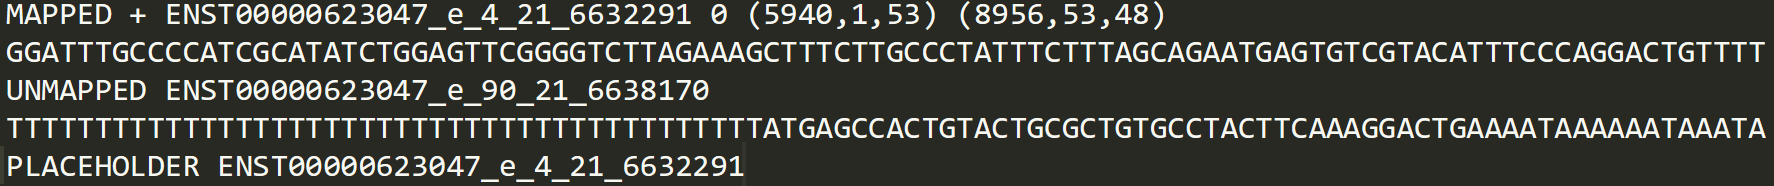
\includegraphics[width=\linewidth]{images/tipiMEM2.png}
  \caption{I diversi tipi di MEM}
  \label{fig:MEMTypes}
\end{figure}

\newpage

\subsection{Supporto alle fragment library types}
Ci sono diversi protocolli per la preparazione di librerie paired-end, che portano a read con caratteristiche diverse. Le \textbf{fragment library types} permettono di descrivere queste caratteristiche in modo sintetico. Le caratteristiche che possono essere descritte sono:
\begin{itemize}
	\item \textbf{Orientamento relativo di una read rispetto all'altra}: può essere inward (I) o outward (O)
	\item \textbf{Se è noto o meno lo strand di appartenenza delle due read}:  può essere stranded (S) o unstranded (U)
	\item \textbf{La direzionalità della prima read, solo nel caso stranded}: può essere first (F) o reverse (R)
\end{itemize}

La seguente immagine descrive tutte le possibili combinazioni:
\begin{figure}[h]
	\centering
	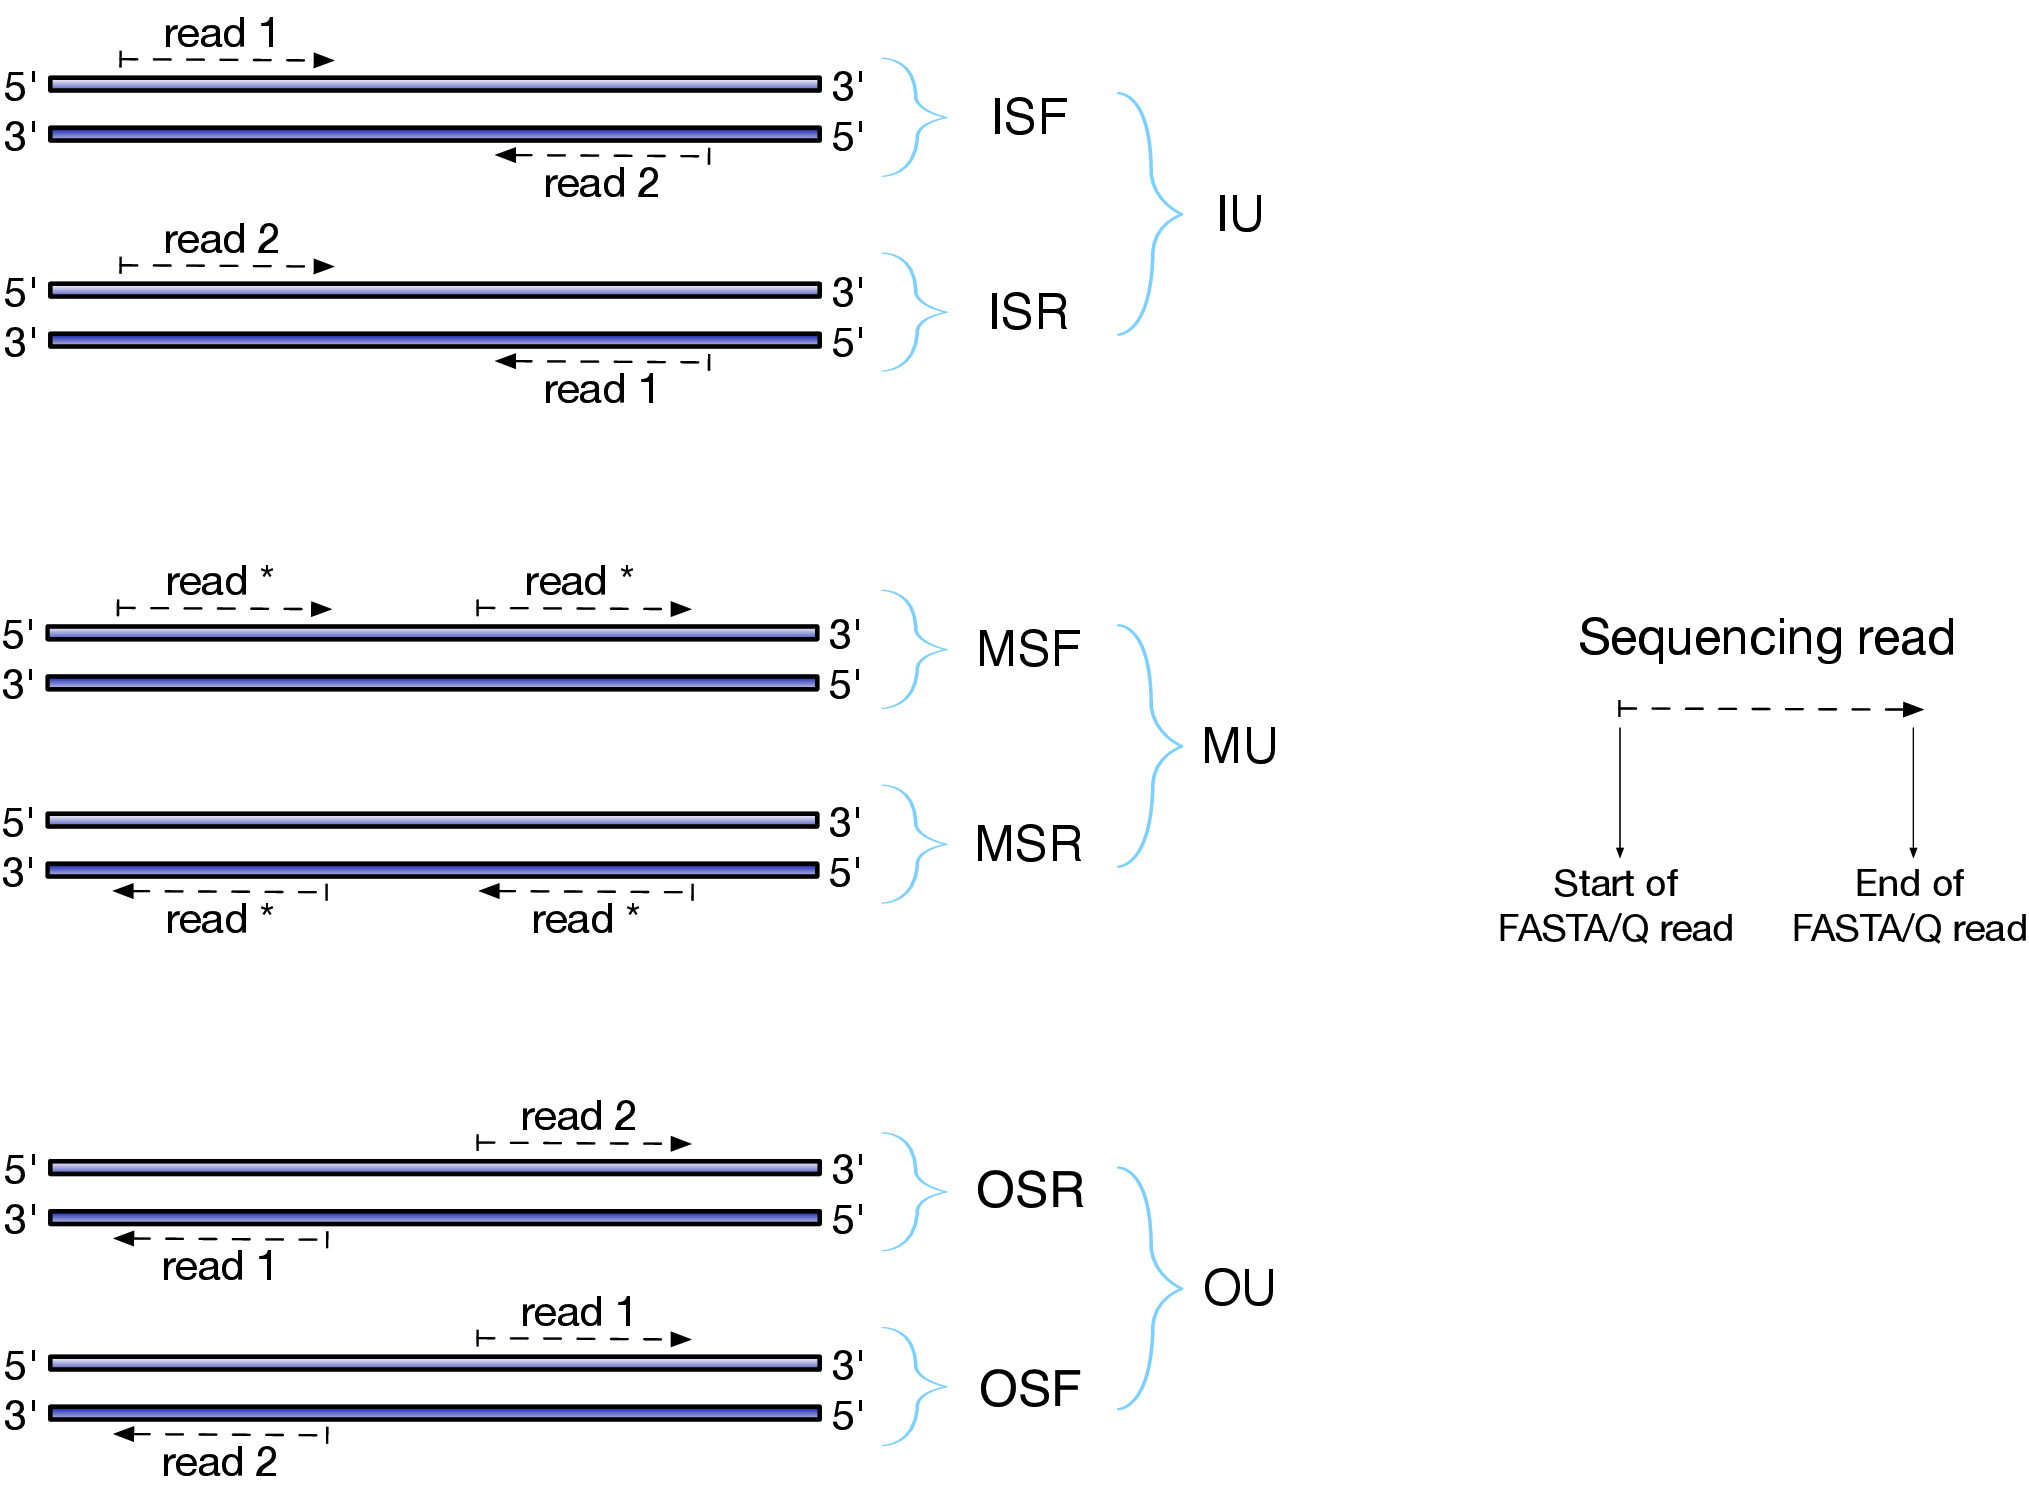
\includegraphics[width=\linewidth]{images/fragmentlibrarytypes.png}
  \caption{I diversi tipi di FTL}
  \label{fig:FragmentLibraryTypes}
\end{figure}

\newpage

ASGAL utilizza queste informazioni per velocizzare il processo di allineamento. Nel formato single-end questa informazioni non esiste, quindi ogni read veniva allineata in entrambe le direzioni, e si prendeva l'allineamento migliore dei due. 

Nel formato paired-end, si può utilizzare la ftl per ridurre il numero di allineamenti necessari, fino al 50\% nel caso stranded. Ad esempio, se viene fornita un ftl di tipo ISF è sufficiente allineare la read 1 sullo strand + (ignorando lo strand -) e la read 2 sullo strand - (ignorando lo strand +).

Il caso unstranded richiede un po' più di attenzione: non è infatti possibile sapere a priori su quale strand allineare la prima read. Per risolvere questo problema è stata riutilizzata la vecchia procedura di allineamento della prima read in entrambe le direzioni; una volta trovata la direzione migliore per la prima, la seconda viene di conseguenza. 

Supponiamo ad esempio di avere una libreria in formato MU: se la prima read allinea sullo strand +, di conseguenza anche la seconda sarà allineata sullo strand +; viceversa, se la prima read allinea sullo strand -, anche la seconda allinea sempre sullo strand -. In questo caso si ottiene solo una riduzione del 25\% nel numero degli allineamenti.

Qualora il tipo di libreria non venga fornito dall'utente, rimane necessario provare ad allineare le read in entrambe le direzioni, senza alcuni incremento di prestazioni.


